\documentclass[12pt,letterpaper]{article}
\usepackage{lipsum}
\usepackage[margin=1in]{geometry}
\usepackage{amsmath}
\usepackage{amssymb}
\usepackage{indentfirst}
\usepackage{setspace}
\usepackage{graphicx}
\usepackage{caption}
\usepackage{pdfpages}
\usepackage{float}
\usepackage{multicol}
\usepackage{enumitem}


\usepackage[citebordercolor={1 1 1}, linkbordercolor={1 1 1}, filebordercolor={1 1 1}]{hyperref}

\linespread{1.25}
	\numberwithin{equation}{section}
	
\begin{document}

\begin{titlepage}

	\begin{center}
	\begin{spacing}{1.0}

		\vspace*{0.6in}
		\huge{\bfseries Rubik's Cubes}\\
			[2mm]
		\huge{\bfseries Influence of Scrambling Method on Solve Difficulty}\\
			[10mm]
		\textsc{\large ECE 302 End of Course Project}\\
			[2.0in]
	
		\line(1,0){450}\\
			[0.5in]
		\textsc{\large Matthew Patrohay}\\
		\textsc{\large ECE 302}\\
		\textsc{\large December 1st, 2023}\\
			[0.5in]
		\textsc{\large Purdue University}\\
			[0.5in]

			
		\line(1,0){450}\\
	\end{spacing}
	\end{center}
	
\end{titlepage}
\newpage
\tableofcontents

%------------------------------------------------------------------------------------------------------------- 		Introduction START               ----------------------------------------------------------------------------------------------------------- 

\newpage

\section{Background}

Before I get into the primary purpose of the project (assessing the solving difficulty of different scrambling approaches) I feel it necessary to first provide a brief introduction of miscellaneous relevant information. 

\subsection{About Speedsolving}

Most have heard of the Rubik's Cube, many know that some people are exceptionally good at solving one, but few know how seriously the hobby/sport is taken. There exists an extensive community of competitive "speedcubers" that all compete to solve the Rubik's Cube as quickly as possible in formal competitions hosted and regulated by the World Cube Association (WCA). Competitions involve various categories, including different cube sizes and restricted solving methods, such as solving with one hand or blindfolded. The appeal of speedcubing lies in its blend of mental challenge, dexterity, and the thrill of achieving faster times through practice and skill refinement.

\subsection{What is A Scramble?}

Before delving deeper, it's essential to understand how a Rubik's Cube functions and what a "scramble" is. A Rubik's Cube is a 3D puzzle consisting of smaller, colored "cubelets" that rotate around three axes. Each face of the cube can be independently rotated, thus, mixing the colors. A "scramble" refers to a sequence of moves, denoted by letters (Singmaster notation), applied to the cube to reach a particular configuration, or "cube state," starting from a solved state; more specifically, a a scramble should result in a cube state that is unknown to a competitor and sufficiently mixed up to avoid obvious solutions. The scrambling process ensures that each solve begins with a unique challenge. A visual representation of the standard turn notation is provided below. 

	\begin{figure}[H]
		\centering
		 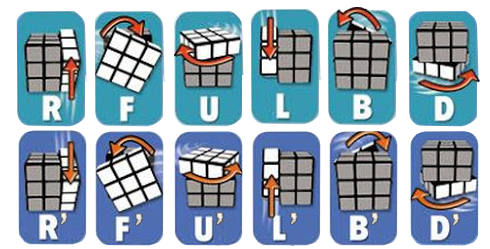
\includegraphics[width=2.75in]{complete-cube-notations.png}
		 \caption{Common Singmaster Notation}
		 \label{fig:turn_notation}
	\end{figure}

\subsection{Importance of Scramble Generation}
Unfortunately, however, an inherent aspect of luck is involved due to the nature of the Rubik's Cube itself. Each scramble can result in a cube configuration that may be inherently easier or more difficult to solve, depending on the sequence of moves required. This randomness adds an element of luck, as a solver might get a 'lucky scramble' leading to exceptionally fast solving times, or conversely, a more complex scramble that requires more time to resolve. To generally address this issue, competitions are organized such that for any given competition all competitors solve the exact same scrambles. This makes each individual competition "fair" as the playing-field is the same for all competitors. However, there can still exist discrepancy across different competitions, making it hard to keep a fair global world-record/ranking leaderboard. Therefore, it is imperative that each of the scrambles given to competitors is generated (using standardized computer code) in a completely random and fair manner.


\section{Scrambling Methods}
Speedcubing bears a resemblance to chess in that a participant's performance is heavily influenced by their investment in practice. Considering the Rubik's Cube's virtually limitless permutations, the most effective strategy for competition preparation is extensive practice. This involves engaging with as many cube configurations as possible, allowing cubers to familiarize themselves with recurring patterns and strategic concepts that can enhance their solving techniques. Serious competitors often turn to apps that generate scramble sequences, which they apply to their cubes to practice solving under competition-like conditions.

My personal interest in this topic comes from the development of one such practice app. The method of scramble generation is a critical aspect that users take seriously. As the app's developer, I am faced with a pivotal decision regarding the scramble generation method. This paper delves into two prevalent methods: 'Random Turns' and 'Random Cube State.' Each method has its implications on the fairness and variability of scrambles, a factor crucial for simulating realistic competition scenarios and aiding in effective practice.

\subsection{Random Turns | Scramble Approach}
This is a very simple and intuitive scrambling approach, and likely what most would assume is the standardized approach to a fair scramble. You simply list out all the possible turns (R, R', L, L', U, U', D, D', F, F', B, B') and randomly select, say, 15 of them and consider it sufficiently randomly scrambled. 

The Random Turns scramble approach is straightforward and intuitive and often perceived as the standard method for achieving a fair scramble in speedcubing. In this method, all possible turns on a Rubik's Cube are first enumerated (R, R', L, L', U, U', D, D', F, F', B, B'), then, to generate a scramble, a specific number of these moves (commonly around 15 to 20) is randomly selected from this pool. This sequence is then applied to a solved cube, resulting in a scrambled state. The rationale behind this approach is that by randomly choosing from all possible moves, the cube will reach a sufficiently randomized state, helping to ensure that no particular pattern or solution is favored. This is, essentially, the same way a human may attempt to scramble a Rubik's cube to the best of their ability (assuming you could actually perform true random moves, which humans are not particularly good at in reality).

\subsection{Random Cube State | Scramble Approach}
This is a significantly more complex scrambling method and is the official scramble approach as regulated by the World Cube Association. A rubiks cube, as briefly stated in the introduction, is comprised of individual pieces called "cubelets" (twelve edge cubelets with 2 faces each, eight corner cubelets with 3 faces each, and six center cubelets with 1 face each). The "Random Turns" approach is effectively just randomizing the turns applied to the cubelets, whereas the goal of the "Cube State" approach is to randomize the final position of each cubelet in the scrambled state. A simple visual is to imagine taking apart a rubiks cube piece by piece, mixing together all the pieces, and putting them all back together randomly. However, generating a "scramble sequence" that uses this approach is more difficult than you might think. Here is the general (simplified as the details aren't relevant) approach for how it is done:

\begin{enumerate}
    \item \textbf{Generate a Random Cube State:} This step really isn't too difficult, as it truly is similar to taking apart the cube and putting it back randomly (in code this is typically represented as an array of piece colors). The only issue is that not all orientations of the individual pieces result in a cube that is even possible to solve, so there are a few logical checks that need to be made to ensure that the cube remains solvable. 

    \item \textbf{Solve the Randomized State:} This step is how the turns associated with the random state are determined. Essentially, take the randomized cube state and solve it while recording all the turns that were performed along the way (Similar to the random turns approach, this is typically about 20 turns). This step is, understandably, very computationally expensive. If you're curious, this is typically achieved via some variation of Kociemba's algorithm which you can read about on wikipedia under "Optimal solutions for the Rubik's Cube".

    \item \textbf{Inverse the Solution for the Scramble Sequence:} Essentially, if you just undo every move in the solution from step 2, you can go from the solved state back to the original scramble that was generated in step 1 (in this case the random cube state). That is to say, if you reverse the order of the solution (and inverse the direction of the turn | clockwise becomes counterclockwise and vice versa) then you get a scramble that would turn a solved cube into the randomized cube state that was generated in step 1.
\end{enumerate}

\section{Purpose of the Paper}
After over three pages of background on Rubik's Cubes (sorry) it is finally time to talk about what I hope to analyze: There exists a common opinion among speedcubers that the Random Turns approach to scrambling a cube results in significantly easier scrambles than the Random Cube State approach. My goal is to test this perceived difference by simulating the solving process on thousands of solves to see if there is any definitive difference. 

\section{Procedure}
The general approach is to generate 1000 scrambles for each scrambling method, then put each scramble through a human-method Rubik's cube solving program to simulate the number of turns a human would take to solve the cube. 
\subsection{Scramble Generation | Random Turns}
To generate the random scrambles for the Random Turns method, I wrote a fairly simple python program that would randomly select a sequence of turns. The big question here is how many turns I should randomly generate, as, in theory, that should correlate with the difficulty of the scramble. I believe the most fair length would be 20 turns, as this is approximately the length that each random cube state scramble ends up being. However, I went ahead and did a range of scramble lengths (10, 15, 20, 25, 30, and 35 turns) this way I can also see the influence of the number of turns on scramble difficulty. 

\subsection{Scramble Generation | Random Cube State}
To generate the Random Cube State scrambles, I used an open source python package called "pyTwistyScrambler". It's essentially just a wrapper package for the most commonly used open source scramble library that was originally written in JavaScript. While this is technically not the "Official" program used by the WCA in competitions, it still follows all the regulations set in place by them (Their program is available, its just in an obscure and slow language). keep in mind, I cant do a range of turn length options here like the Random Turns scrambles, as the length here is determined by the number of turns the Kociemba algorithm takes to generate the scramble.  

\subsection{Solve the Cube | Human-Method Program}
After 1000 of each of the scrambles have been generated, I put all of them through a program that attempts to solve the Rubik's cube the way a human would. The program I used was written by a Harvard student for their CS50x final project in 2021 and can be found here (https://github.com/d4m4s74/Cube-Solver). The solving approach they used is called CFOP, and is the most common (and typically fastest) method used by speedcubers in competition. I then recorded the total number of turns required for each solve. Additionally, for my own curiosity, I also separated each solve into its four primary components (CFOP has four primary steps: Cross, F2L, OLL, and PLL) to see the influence of each scramble method on each individual step during solving. 

\subsection{Analysis of Solve Data}
The primary analysis I intend to cover will utilize discrete expected value calculations to assess the solve difficulty for each scrambling method. First, I must define the random variable, X, as the number of turns required to solve the Rubik's cube for any given method. Then, given the data collected from 1000 simulated solves for each scramble method, I will construct histograms to visualize the distribution of turns required in each scenario. These histograms serve as the basis for deriving the probability mass function (pmf), denoted as $p_X(x)$. The pmf will provide a detailed probabilistic breakdown of the number of turns needed for solving the cube across different scramble methods.

The expected value, $E[X]$, is then calculated using the formula:

\begin{equation}
E[X] = \sum_{x \in R_X} x \cdot p_X(x)
\end{equation}

This equation essentially computes the weighted average of turns needed, where the weights are the probabilities of each turn count occurring. This approach will offer a quantitative measure to compare the efficiency and challenge presented by the 'Random Turns' and 'Random Cube State' methods.

To further deepen the analysis, I will also examine the variance and standard deviation of the number of turns for each method. Variance will provide insight into the consistency of the solve difficulty across scrambles, while standard deviation will offer a measure of how spread out the number of turns is from the average. 

The equations for each of the following values are provided below:

\begin{equation}
\text{Var} \left( X\right)  =E\left[ X^{2}\right]  -\left( E\left[ X\right]  \right)^{2}  
\end{equation}
\begin{equation}
\text{Stdev} \left( X\right)  =\sqrt{\text{Var(X)} } =\sqrt{E\left[ X^{2}\right]  -\left( E\left[ X\right]  \right)^{2}  } 
\end{equation}


\section{Results}




\end{document}

